%%%%%%%%%%%%%%%%%%%%%%%%%%%%%%%%%%%%%%%%%%%%%%%%%%%%%%%%%%%%%%%%%%%%%
% LaTeX Template: Praxisprojekt WS 2017
%
% Date: November 2017
%
%%%%%%%%%%%%%%%%%%%%%%%%%%%%%%%%%%%%%%%%%%%%%%%%%%%%%%%%%%%%%%%%%%%%%%

\documentclass[12pt]{article}
\usepackage[a4paper]{geometry}
\usepackage{framed}
\usepackage[myheadings]{fullpage}
\usepackage{fancyhdr}
\usepackage{lastpage}
\usepackage{graphicx, wrapfig, subcaption, setspace, booktabs}
\usepackage[T1]{fontenc}
\usepackage[font=small, labelfont=bf]{caption}
\usepackage[protrusion=true, expansion=true]{microtype}
\usepackage[german]{babel}
\usepackage{sectsty}
\usepackage{url, lipsum}
\usepackage[parfill]{parskip}
\usepackage{listings}

%-------------------------------------------------------------------------------
% Commands
%-------------------------------------------------------------------------------
\newcommand{\HRule}[1]{\rule{\linewidth}{#1}}
\input{env}
%-------------------------------------------------------------------------------
% HEADER & FOOTER
%-------------------------------------------------------------------------------
\pagestyle{fancy}
\fancyhf{}
\setlength\headheight{15pt}
\fancyhead[L]{\newCommandName}
\fancyhead[R]{\newCommandUniversity}
\fancyfoot[R]{Seite \thepage\ von \pageref{LastPage}}

%-------------------------------------------------------------------------------
% TITLE PAGE
%-------------------------------------------------------------------------------
\begin{document}


\title{ \normalsize
		\HRule{0.5pt} \\
		\LARGE \textbf{\uppercase{\newCommandDiscipline}} \\
		\smallbreak
		\small\textbf{{\newCommandTerm}}\\
		\HRule{2pt} \\ [0.5cm]
		\normalsize \today \vspace*{10\baselineskip}}

\date{}

\author{
		\newCommandName \\
		\newCommandMatriculationNumber \\
		\newCommandUniversity \\
		\newCommandFaculty
}

\pagenumbering{gobble}

\maketitle

\newpage

\pagenumbering{arabic}


%-------------------------------------------------------------------------------
% Section title formatting
\sectionfont{\scshape}
%-------------------------------------------------------------------------------

%-------------------------------------------------------------------------------
% BODY
%-------------------------------------------------------------------------------

\section{Statusbericht}
\subsection{Was habe ich bisher im Projekt erreicht?}
\begin{itemize}
\item Security abgeschlossen - Kong Api-Gateway etabliert
\item S3 abgeschlossen - Minio Objectstorage
\item Job-Mock entworfen (Fibonacci - ``intentionally slow'')
\item Architecture High-Level definiert
\item Swagger getestet und Funktionalitaet adaptiert
% \item Automatisierung in der Entwicklungsumgebung implentiert
\end{itemize}
\smallbreak

\begin{figure}[!htp]
	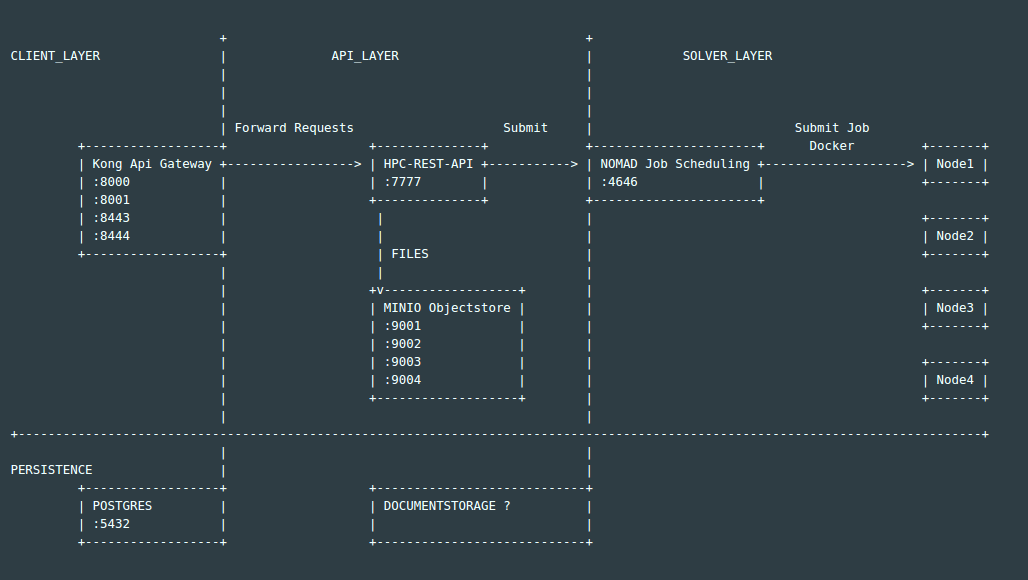
\includegraphics[width=1\textwidth]{./img/Architecture.png}
	\captionsetup{name=Abb.,font=footnotesize}
	\caption{Architecture High-Level}
	% \centering
\end{figure}

\subsection{Was habe ich bis zum n"achsten Statusbericht vor?}


\begin{itemize}
\item Kompletter Durchlauf der Api-Architectur
\begin{itemize}
	\item 1. Job erstellen
	\item 2. Job submitten
	\item 3. Solver Gateway - Nomad Scheduling of Jobs
	\item 4. Send Results back to client
\end{itemize}
\item Spezifizieren der Api (analog Rescale Api)
\item Dokumentation der Api
\item Persistence-Layer der Api (Jobs und deren Results werden in einer Datenbank gespeichert)
\end{itemize}

Dokumentation der Issues werden direkt im Repository gef"uhrt.
\subsection{Gibt es Probleme bei der Durchf"uhrung?}
\begin{itemize}
\item Es gab Probleme mit Swagger so dass ich die Umsetzung mit Hilfe dessen verworfen habe. Die Komplexit"at des generierten Codes war zu hoch. Ich denke ich mache es ``completely from scratch''.
\end{itemize}


\section{Ressourcen}
\textbf{Git-Repository als Versionskontrolle:}\\
\url{https://github.com/MatthiasHertel/ws17_pp}

\textbf{Webseite zur Dokumentation:}\\
\url{https://www.ws17-pp.mhertel.de}


\end{document}
